\documentclass{beamer}
\usepackage{amsmath, amssymb}
\usepackage{graphicx}
\usepackage{listings}
\usepackage{color}
\usepackage{subfig}
\usepackage{hyperref}
\usepackage{fancyvrb}



\title{Mixed Effects Models - Day 7}
\subtitle{Diagnostics of Mixed Effects Models}
\author{Marieke Wesselkamp\\Department of Biometry and Environmental Systems Analysis\\Albert-Ludwigs-University of Freiburg (Germany)}
\date{February 2023}

\begin{document}

\frame{\titlepage}

\begin{frame}
    \frametitle{The Linear Mixed Effects Model}
    \[
    \mathbf{y} = \mathbf{X} \cdot \mathbf{b} + \mathbf{Z} \cdot \mathbf{u} + \mathbf{e}
    \]
    \[
    \mathbf{e} \sim \mathcal{N}(0, \mathbf{R}), \quad \mathbf{u} \sim \mathcal{N}(0, \mathbf{G}), \quad \mathbf{u} \bot \mathbf{e}
    \]
    where:
    \begin{itemize}
        \item $\mathbf{y}$: measured response values
        \item $\mathbf{X}$: Fixed Effects design matrix
        \item $\mathbf{b}$: Fixed Effects parameter vector of $\mathbf{X}$
        \item $\mathbf{e}$: Vector of the errors $\epsilon$, which are normally distributed (mean = 0; variance by residual variance-covariance matrix \textbf{R})
    \end{itemize}
\end{frame}

\begin{frame}
    \frametitle{Stochastic Components of Mixed Effects Models}
    \begin{itemize}
        \item The \textbf{first stochastic part} describes how random effects parameters $\mathbf{u}$ vary around 0 and is given by the random effects variance-covariance matrix \textbf{G}
        \[
        \mathbf{u} \sim \mathcal{N}(0, \mathbf{G})
        \]
        \item The \textbf{second stochastic part} describes the remaining and unexplained (\textit{residual}) variance:
        \[
        \mathbf{e} \sim \mathcal{N}(0, \mathbf{R})
        \]
        It describes how the measurements \textbf{e} vary around 0, \textbf{After} accounting for the fixed and random effects and is given by the residual variance-covariance matrix \textbf{R}.
    \end{itemize}
\end{frame}

\begin{frame}
    \frametitle{Assumptions of Mixed Effects Models}
    \begin{enumerate}
        \item $\mathbf{b}$ describes the deterministic trend averaged over the random effects $\mathbf{u}$.
        \item Random effects $\mathbf{u}$ are normally and independently distributed among groups with $\mathit{mean = 0}$ and covariance matrix $\mathbf{G}$.
        \item Residual errors $\mathbf{e}$ are normally and independently distributed within a group with $\mathit{mean = 0}$ and variance $\sigma^2$.
        \item $\mathbf{u}$ and $\mathbf{e}$ are independent of each other: among groups, there are no correlation of errors 
        \item Variances and covariances do not depend on group: they are homogeneous, each group has the same values.
    \end{enumerate}
\end{frame}

\begin{frame}
    \frametitle{Assumptions of Mixed Effects Models}
    \begin{enumerate}
        \item $\mathbf{b}$ describes the deterministic trend averaged over the random effects $\mathbf{u}$.
        \item Random effects $\mathbf{u}$ are normally and independently distributed among groups with $\mathit{mean = 0}$ and covariance matrix $\mathbf{G}$.
        \item Residual errors $\mathbf{e}$ are normally and independently distributed within a group with $\mathit{mean = 0}$ and variance $\sigma^2$.
        \item $\mathbf{u}$ and $\mathbf{e}$ are independent of each other: among groups, there are no correlation of errors 
        \item Variances and covariances do not depend on group: they are homogeneous, each group has the same values.
    \end{enumerate}
    \vspace{0.2cm}
    
    \textbf{Violations of these assumptions can lead to problems with residuals and fitting. Each assumption must be tested.}
\end{frame}

\begin{frame}
    \frametitle{Model Specification: Key Components}
    \textbf{The key to a well behaved model is to specify your model correctly. For MEMs there are three parts to be specified:}
    \vspace{0.2cm}
    
    \begin{itemize}
        \item The fixed (deterministic) effects part
        \item The random effects part
        \item The residual variance part
    \end{itemize}
\end{frame}

\begin{frame}
    \frametitle{The recipe to a good model}
    \begin{itemize}
        \item[] \textbf{True for all models:}
        \item define the deterministic part of the model, i.e. find the fixed effects incl. their interactions and potential quadratic / cubic etc. terms.
        \item choose a distribution for the errors
        \item[] 
        \item[] \textbf{Additionally for Mixed Effect Models:}
        \item spot the grouping in the data
        \item how many random effects are there in the data?
        \item if two or more, are they nested or crossed?
        \item can you specify random slopes / random contrasts for one or all of the random effects?
    \end{itemize}
\end{frame}

\begin{frame}[fragile]
    \frametitle{}
    \textbf{The idea of a \color{blue}{sick}} \textbf{model also applies to Mixed Effect Models}
    \vspace{0.2cm}
    \begin{center}
        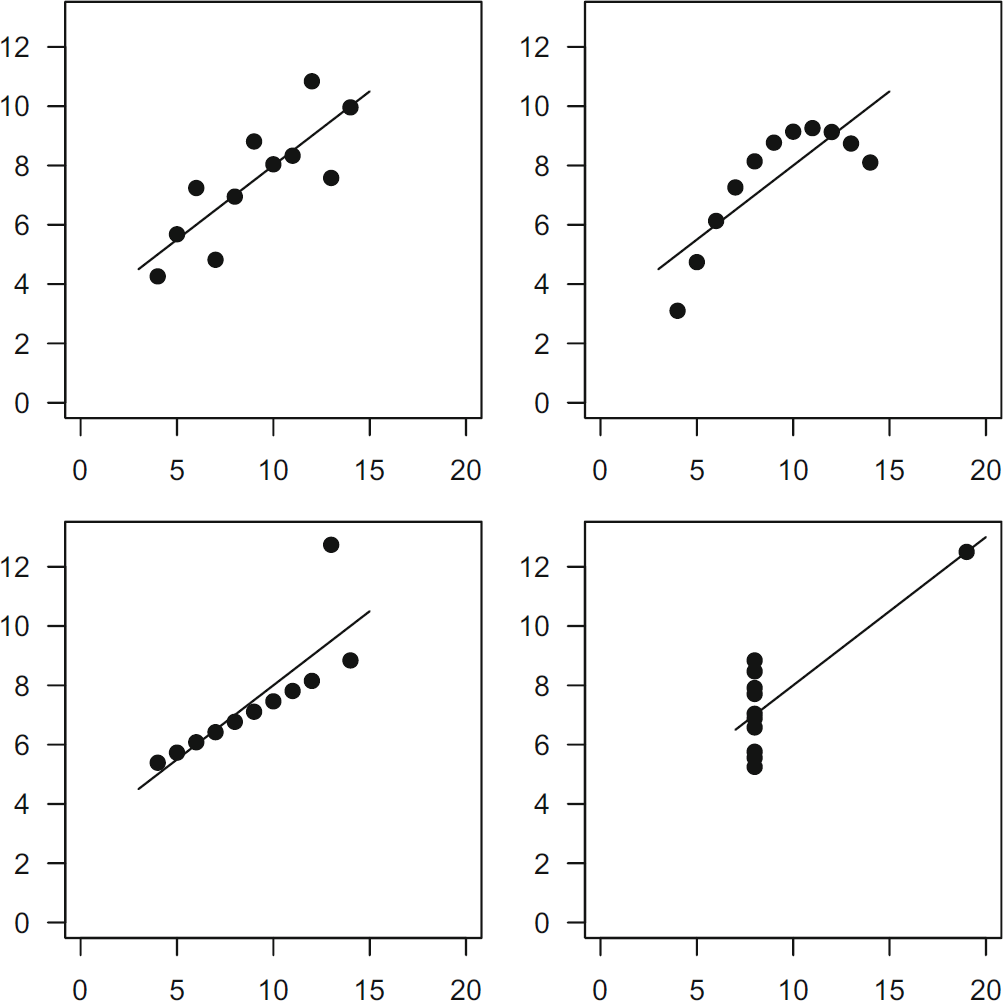
\includegraphics[width=0.6\textwidth]{lectures/day_7_diagnostics_of_mems/figures/Anscombe.png}
    \end{center}
\end{frame}

\begin{frame}
    \frametitle{Residual Checks for LMEMs}
    \begin{center}
    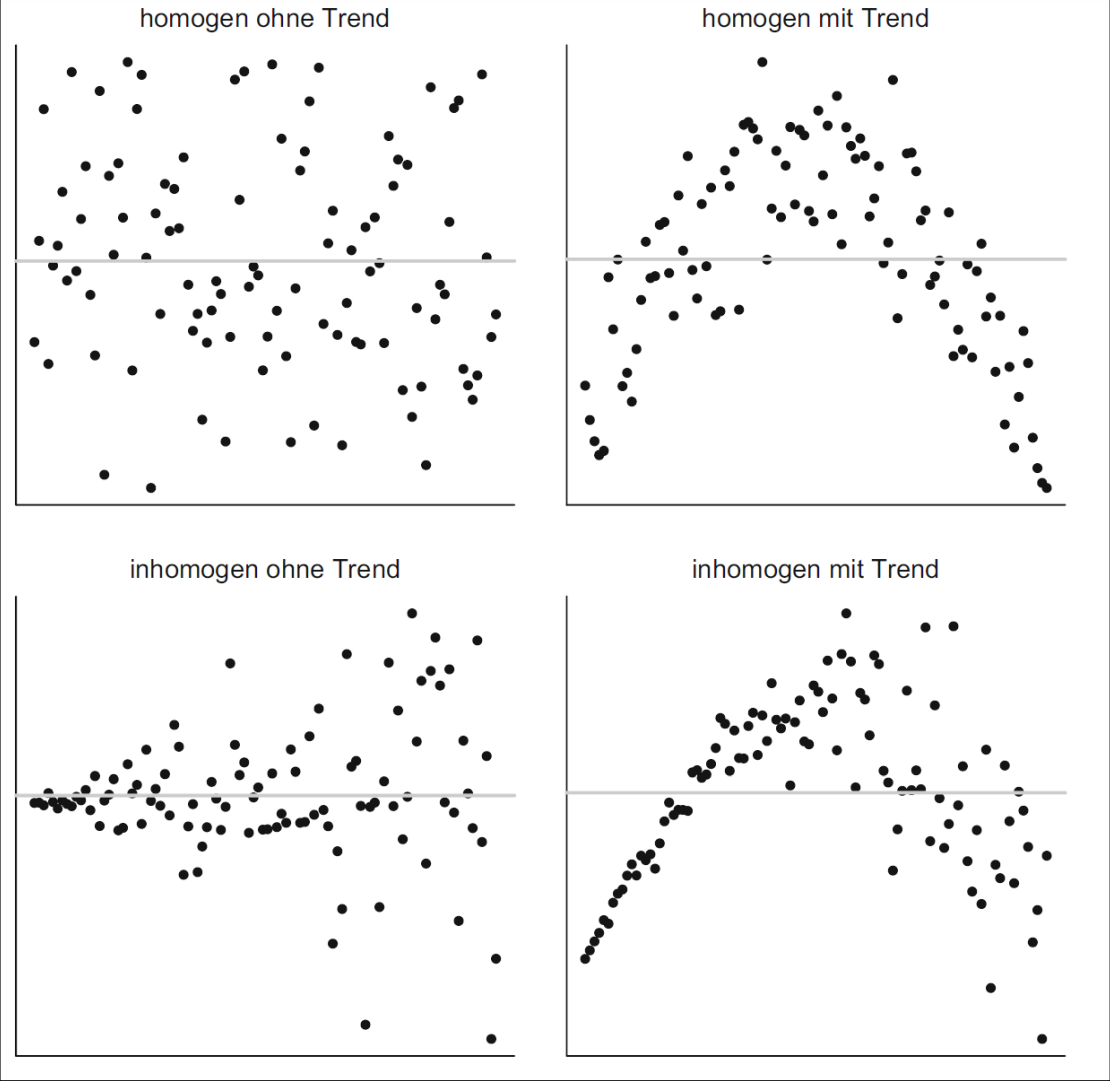
\includegraphics[width=0.6\textwidth]{lectures/day_7_diagnostics_of_mems/figures/residuals.png}    
    \end{center}
    \textbf{Linear Mixed Effects Models (LMEMs) require more checks because they have more assumptions!}
\end{frame}

\begin{frame}
    \frametitle{}
    \huge\color{purple}\textbf{1. Check the Grouping in the Output}
    \vspace{0.5cm}
    
    \normalsize\color{black}\textbf{Example: Glycogen concentration measurements from a nested design involving rats, livers, and preparation methods.}
\end{frame}

\begin{frame}[fragile]
    \frametitle{}
    \begin{columns}
        \begin{column}{0.5\textwidth}
            In 3 treatments the liver of 2 rats each were cut into 3 pieces and per liver piece 2 preparations for glycogen concentration were obtained\\
            = 3 x 2 x 3 x 2 = 36
        \end{column}
        \begin{column}{0.5\textwidth}
            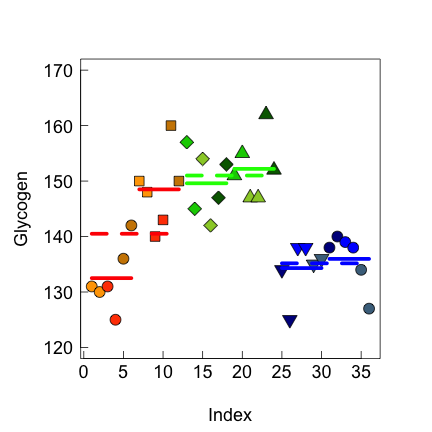
\includegraphics[width=\textwidth]{lectures/day_7_diagnostics_of_mems/figures/unnamed-chunk-3-1.png}
        \end{column}
    \end{columns}
\end{frame}

\begin{frame}[fragile]
    \frametitle{Nested Design}
    \begin{columns}
        \begin{column}{0.6\textwidth}
            \tiny\begin{Verbatim}[numbers=left,numbersep=6pt,frame=single]
m.r <- lmer(Glycogen~Treatment+(1|Rat/Liver), rats)
            \end{Verbatim}
            \scalebox{1}{
                \lstinputlisting[frame=single]{lectures/day_7_diagnostics_of_mems/outputs/output_1.txt}
            }
        \end{column}
        \begin{column}{0.4\textwidth}
            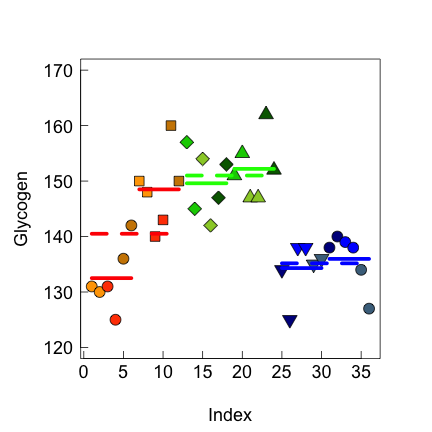
\includegraphics[width=\textwidth]{lectures/day_7_diagnostics_of_mems/figures/unnamed-chunk-3-1.png}
        \end{column}
    \end{columns}
\end{frame}

\begin{frame}[fragile]
    \frametitle{Wrongly Crossed Design}
    \begin{columns}
        \begin{column}{0.6\textwidth}
            \tiny\begin{Verbatim}[numbers=left,numbersep=6pt,frame=single]
m.r.2 <- lmer(Glycogen~Treatment+(1|Rat)+(1|Liver), rats)
            \end{Verbatim}
            \scalebox{1}{
                \lstinputlisting[frame=single]{lectures/day_7_diagnostics_of_mems/outputs/output_2.txt}
            }
        \end{column}
        \begin{column}{0.4\textwidth}
            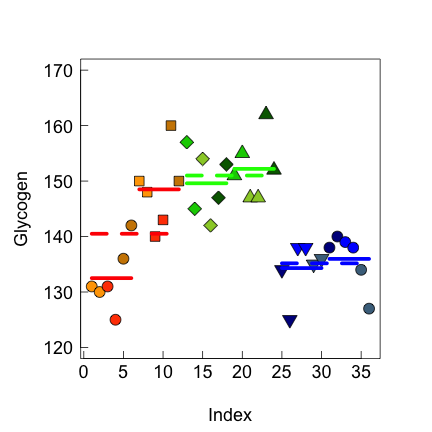
\includegraphics[width=\textwidth]{lectures/day_7_diagnostics_of_mems/figures/unnamed-chunk-3-1.png}
            \textbf{different groupings and different variance components}
        \end{column}
    \end{columns}
\end{frame}

\begin{frame}
    \frametitle{}
    \huge\color{purple}\textbf{2. Check the Variance Components}
    \vspace{0.5cm}
    
    \normalsize\color{black}\textbf{
    A high correlation or singular fit may indicate an issue with model specification.}
\end{frame}

\begin{frame}[fragile]
    \frametitle{}
    \textbf{A correlation of exactly 1 and a singular fit?}
    \tiny
    \begin{Verbatim}[numbers=left,numbersep=6pt,frame=single]
m.f <- lmer(root ~ week * fertilizer + (week|plant), fertilizer)
summary(m.f)        
    \end{Verbatim}
    \scalebox{1}{
        \lstinputlisting[frame=single]{lectures/day_7_diagnostics_of_mems/outputs/output_3.txt}
    }
\end{frame}

\begin{frame}[fragile]
    \frametitle{}
    \tiny
    \begin{Verbatim}[numbers=left,numbersep=6pt,frame=single]
m.f.no <- lmer(root ~ week * fertilizer + (week||plant), fertilizer)
summary(m.f.no) 
    \end{Verbatim}
    \scalebox{1}{
        \lstinputlisting[frame=single]{lectures/day_7_diagnostics_of_mems/outputs/output_4.txt}
    }
    \vspace{}
    
    \normalsize
    \textbf{Of course that is not “keeping it maximal”, but as maximal as possible}
\end{frame}

\begin{frame}
    \frametitle{}
    \huge\color{purple}\textbf{3. Check Normality of Random Effects}
    \vspace{0.5cm}
    
    \normalsize\color{black}\textbf{Use visual tools such as histograms and QQ plots to check for normality.}
\end{frame}

\begin{frame}[fragile]
    \frametitle{}
    \textbf{We use the model without correlation}
    \vspace{0.5cm}
    
    \scriptsize
    \begin{Verbatim}[numbers=left,numbersep=6pt,frame=single]
m.f.2 <- lmer(root ~ week * fertilizer + (week||plant), fertilizer)
VarCorr(m.f.2)         
    \end{Verbatim}
    \scalebox{1}{
        \lstinputlisting[frame=single]{lectures/day_7_diagnostics_of_mems/outputs/output_5.txt}
    }
\end{frame}

\begin{frame}[fragile]
    \frametitle{Random Intercept Check}
    \begin{columns}
        \begin{column}{0.45\textwidth}
            \textbf{Plotting}
            \scriptsize
            \begin{Verbatim}[numbers=left,numbersep=6pt,frame=single]
hist(ranef(m.f.2)$plant[,1])
            \end{Verbatim}
            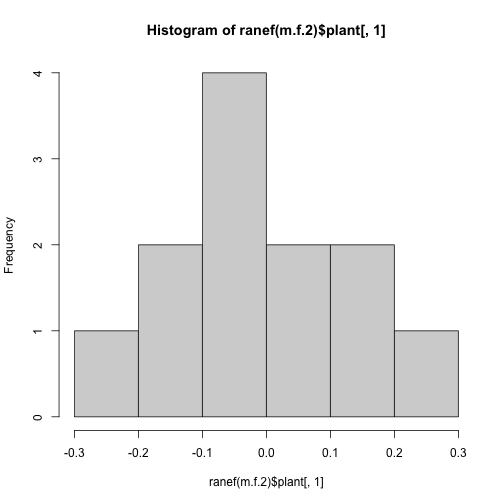
\includegraphics[width=\textwidth]{lectures/day_7_diagnostics_of_mems/figures/unnamed-chunk-14-1.png}
        \end{column}
        \begin{column}{0.55\textwidth}
            \textbf{Testing}
            \scriptsize
            \begin{Verbatim}[numbers=left,numbersep=6pt,frame=single]
shapiro.test(ranef(m.f.2)$plant[,1])
            \end{Verbatim}
            \scalebox{1}{
                \lstinputlisting[frame=single]{lectures/day_7_diagnostics_of_mems/outputs/output_6.txt}
            }
        \vspace{1.45cm}
        
        \normalsize\textbf{
        The Shapiro-Wilk test tests for a significant difference of the data distribution to normality, i.e. if $\mathit{p}<0.05$, the data are not normal.}
        \end{column}
    \end{columns}
\end{frame}

\begin{frame}[fragile]
    \frametitle{Random Slope Check}
    \begin{columns}
        \begin{column}{0.45\textwidth}
            \textbf{Plotting}
            \scriptsize
            \begin{Verbatim}[numbers=left,numbersep=6pt,frame=single]
hist(ranef(m.f.2)$plant[,2])
            \end{Verbatim}
            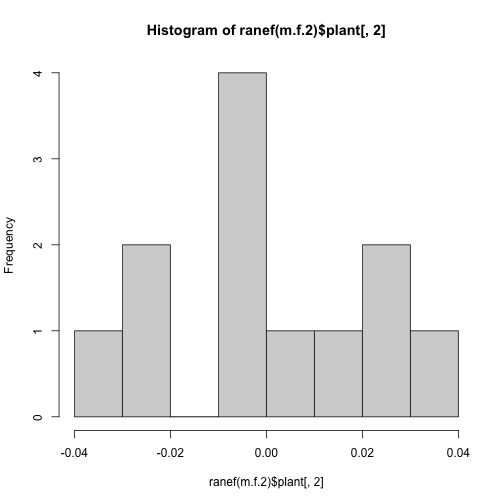
\includegraphics[width=\textwidth]{lectures/day_7_diagnostics_of_mems/figures/unnamed-chunk-16-1.png}
        \end{column}
        \begin{column}{0.55\textwidth}
            \textbf{Testing}
            \scriptsize
            \begin{Verbatim}[numbers=left,numbersep=6pt,frame=single]
shapiro.test(ranef(m.f.2)$plant[,2])
            \end{Verbatim}
            \scalebox{1}{
                \lstinputlisting[frame=single]{lectures/day_7_diagnostics_of_mems/outputs/output_7.txt}
            }
            \vspace{3.25cm}
            
        \end{column}
    \end{columns}
\end{frame}

\begin{frame}[fragile]
\frametitle{Another useful perspective: QQ-Plots}
    \begin{columns}
        \begin{column}{0.5\textwidth}
        \textbf{Intercept ranefs}
        \scriptsize
            \begin{Verbatim}[numbers=left,numbersep=6pt,frame=single]
qqmath(ranef(m.f.2)$plant[,1], 
panel = function(x, ...) {
          panel.qqmathline(x, ...)
          panel.qqmath(x, ...)
       })                
            \end{Verbatim}
            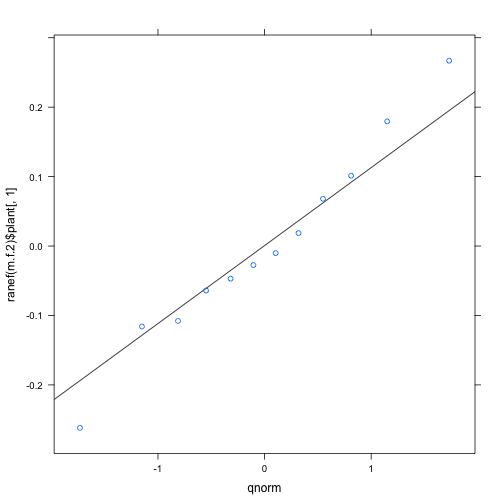
\includegraphics[width=\textwidth]{lectures/day_7_diagnostics_of_mems/figures/unnamed-chunk-18-1.png}
        \end{column}
        \begin{column}{0.5\textwidth}
        \textbf{Slope ranefs}
        \scriptsize
            \begin{Verbatim}[numbers=left,numbersep=6pt,frame=single]
qqmath(ranef(m.f.2)$plant[,2], 
panel = function(x, ...) {
          panel.qqmathline(x, ...)
          panel.qqmath(x, ...)
       })               
            \end{Verbatim}
            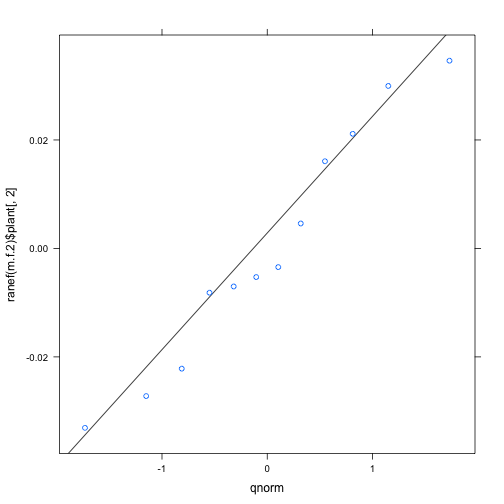
\includegraphics[width=\textwidth]{lectures/day_7_diagnostics_of_mems/figures/unnamed-chunk-19-1.png}
        \end{column}
    \end{columns}
\end{frame}


\begin{frame}[fragile]
    \frametitle{}
    \large\textbf{Note:}\\
    Too few levels of the Random Effects can make these checks difficult.
    \color{violet} e.g. with only 5 genotypes, a distribution is difficult to test.
\end{frame}

\begin{frame}[fragile]
    \frametitle{Random Effects Model: Genotype Deviations}
    \begin{columns}
        \begin{column}{0.5\textwidth}
        \scriptsize
            \begin{Verbatim}[numbers=left,numbersep=6pt,frame=single]
m.g <- lmer(Height ~ poly(P,2) + 
(poly(P,2)|Genotype), geno)
xyplot(Height ~ P|Genotype, geno)                
            \end{Verbatim}
            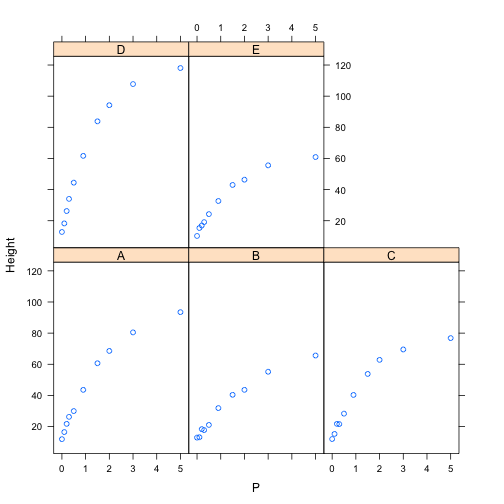
\includegraphics[width=\textwidth]{lectures/day_7_diagnostics_of_mems/figures/unnamed-chunk-21-1.png}
        \end{column}
        \begin{column}{0.5\textwidth}
        \scriptsize
            \begin{Verbatim}[numbers=left,numbersep=6pt,frame=single]
VarCorr(m.g)                
            \end{Verbatim}
            \tiny\scalebox{1}{
                \lstinputlisting[frame=single]{lectures/day_7_diagnostics_of_mems/outputs/output_8.txt}
            }
        \vspace{0.1cm}

        \scriptsize
        \textit{Side Note: see the complex "random slope" here}\\
        \vspace{0.5cm}
        
        \normalsize
        \textbf{Genotype-specific deciations from the non-linear population trend}
        \end{column}
    \end{columns}
\end{frame}

\begin{frame}[fragile]
    \frametitle{Distribution of Random Effects}
    \small\begin{Verbatim}[numbers=left,numbersep=6pt,frame=single]
hist(ranef(m.g)$Genotype[,1])        
    \end{Verbatim}
    \begin{center}
    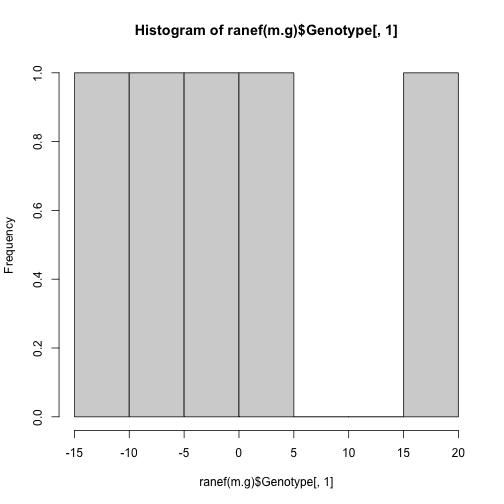
\includegraphics[width=0.65\textwidth]{lectures/day_7_diagnostics_of_mems/figures/unnamed-chunk-23-1.png}        
    \end{center}
\end{frame}

\begin{frame}
    \frametitle{}
    \huge\color{purple}\textbf{4. Check your residuals}
    \vspace{0.5cm}
    
    \normalsize\color{black}\textbf{Revisiting the Orthodont dataset for residual checks.}
\end{frame}

\begin{frame}[fragile]
    \frametitle{Plotting Residuals: Orthodont Data}
    \textbf{Use the in-built plot function for residual plots}
    \scriptsize\begin{Verbatim}[numbers=left,numbersep=6pt,frame=single]
fm1 <- lmer(distance ~ age * Sex + (age|Subject))
plot(fm1)        
    \end{Verbatim}
    \begin{columns}
        \begin{column}{0.5\textwidth}
            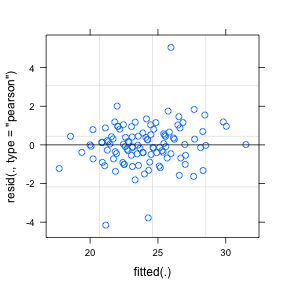
\includegraphics[width=\textwidth]{lectures/day_7_diagnostics_of_mems/figures/unnamed-chunk-25-1.png}
        \end{column}
        \begin{column}{0.5\textwidth}
        \normalsize
            You are looking at all residuals across all fitted values across all predictors and Random Effect levels. There is no strong trend visible.\\
            \textbf{But}, don't jump to conclusions just yet...
        \end{column}
    \end{columns}
\end{frame}

\begin{frame}[fragile]
    \frametitle{QQ Plot of Residuals}
    \scriptsize\begin{Verbatim}[numbers=left,numbersep=6pt,frame=single]
require("lattice")
qqmath(fm1, id=0.05) # set significance level for outlier test        
    \end{Verbatim}
    \begin{columns}
        \begin{column}{0.5\textwidth}
            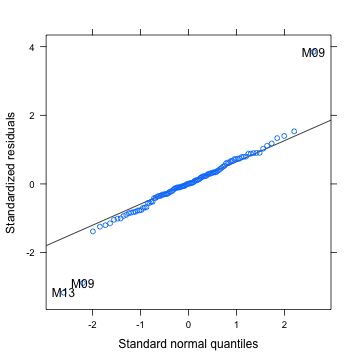
\includegraphics[width=\textwidth]{lectures/day_7_diagnostics_of_mems/figures/unnamed-chunk-26-1.png}  
        \end{column}
        \begin{column}{0.5\textwidth}
        \normalsize
            Here, we look at all residuals across all values and levels of the predictors combined. Three data points seem to deviate quite a bit.
        \end{column}
    \end{columns}
\end{frame}

\begin{frame}
    \frametitle{Residual Plotting Strategy}
    \large
    An overall plot, like the default plots produced above may...
    \vspace{0.2cm}
    
    \begin{itemize}
        \item ... mask any issues
        \item ... show issues, but don't give inside to their origin
    \end{itemize}
    \vspace{0.5cm}
    
    \textbf{Therefore: Subset the residuals in meaningful ways}
\end{frame}

\begin{frame}[fragile]
    \frametitle{Standardized Residuals vs Age}
    \scriptsize\begin{Verbatim}[numbers=left,numbersep=6pt,frame=single]
fm1 <- lmer(distance ~ age * Sex + (age|Subject))
plot(fm1, resid(., scaled=TRUE) ~ age, abline = 0)
    \end{Verbatim}
    \begin{columns}
        \begin{column}{0.5\textwidth}
            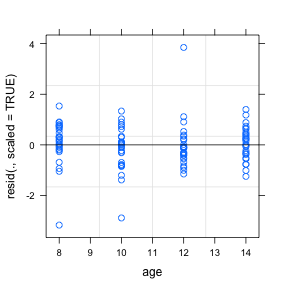
\includegraphics[width=\textwidth]{lectures/day_7_diagnostics_of_mems/figures/unnamed-chunk-27-1.png}
        \end{column}
        \begin{column}{0.5\textwidth}
        \normalsize
            Now you looks at all residuals across all values and levels of the predictor age but NOT sub-setted by Sex or Subject. Possibly some larger variance at ages 8, 10, 12?
        \end{column}
    \end{columns}
\end{frame}

\begin{frame}[fragile]
    \frametitle{Response Residuals vs Fitted Values by Age}
    \scriptsize\begin{Verbatim}[numbers=left,numbersep=6pt,frame=single]
plot(fm1, resid(.) ~ fitted(.) | Sex, abline = 0)
    \end{Verbatim}
    \begin{columns}
        \begin{column}{0.5\textwidth}
            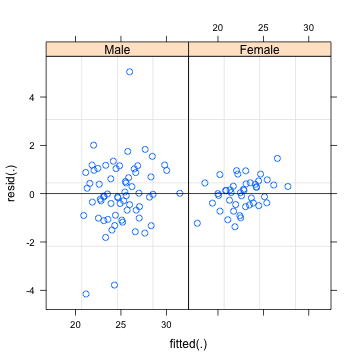
\includegraphics[width=\textwidth]{lectures/day_7_diagnostics_of_mems/figures/unnamed-chunk-29-1.png}
        \end{column}
        \begin{column}{0.5\textwidth}
        \normalsize
            AHA! Here, the spread in residuals is quite a bit larger for boys than for girls: this violates the assumption of homogeneous (constant) variance along a predictor.
        \end{column}
    \end{columns}
\end{frame}

\begin{frame}[fragile]
    \frametitle{Modeling Heterogeneous Residual Variance}
    We could try to model different residual variances for boys and girls (working with the R-side matrix).\\
    e.g. quite easily done with the 'weights' argument in nlme().
    \vspace{0.5cm}

    \scriptsize
    \begin{Verbatim}[numbers=left,numbersep=6pt,frame=single]
mod <- lme(distance ~ age * Sex, random = ~ age|Subject, 
           weights = varIdent(form = ~1|Sex))
getVarCov(mod, type = "random.effects")
    \end{Verbatim}
    \vspace{0.5cm}
    
    \scalebox{1}{
        \lstinputlisting[frame=single]{lectures/day_7_diagnostics_of_mems/outputs/output_9.txt}
    }
\end{frame}

\begin{frame}[fragile]
    \frametitle{Extracting Conditional Variance-Covariance Matrix}
    \scriptsize
    \begin{Verbatim}[numbers=left,numbersep=6pt,frame=single]
getVarCov(mod, individuals = 1, type = "conditional")        
    \end{Verbatim}
    \scalebox{1}{
        \lstinputlisting[frame=single]{lectures/day_7_diagnostics_of_mems/outputs/output_10_1.txt}
    }

    \begin{Verbatim}[numbers=left,numbersep=6pt,frame=single]
getVarCov(mod, individuals = 27, type = "conditional")      
    \end{Verbatim}
    \scalebox{1}{
        \lstinputlisting[frame=single]{lectures/day_7_diagnostics_of_mems/outputs/output_10_2.txt}
    }
\end{frame}

\begin{frame}[fragile]
    \frametitle{}
    \scriptsize
    \begin{Verbatim}[numbers=left,numbersep=6pt,frame=single]
mod
    \end{Verbatim}
    \tiny\scalebox{1}{
        \lstinputlisting[frame=single]{lectures/day_7_diagnostics_of_mems/outputs/output_11.txt}
    }
    \scriptsize
    \begin{Verbatim}[numbers=left,numbersep=6pt,frame=single]
mod$sigma^2*0.4088466^2
---
[1] 0.443889
    \end{Verbatim}
\end{frame}

\begin{frame}[fragile]
    \frametitle{Modeling among-group variances}
    We could also try to model different \textbf{among-group} variances for boys and girls (working with the G-side matrix).
    \vspace{0.5cm}

    \scriptsize
    \begin{Verbatim}[numbers=left,numbersep=6pt,frame=single]
model <- lme(distance ~ age * Sex,
random = list(Subject = pdDiag(form = ~ Sex),
              Subject = pdSymm(form = ~ age)))
    \end{Verbatim}
    \vspace{0.5cm}

    \normalsize
    \textit{pdDiag}: diagonal positive-definite matrix \\
    \textit{pdSymm}: general positive-definite matrix
\end{frame}

\begin{frame}[fragile]
    \frametitle{Extracting among-group variances}
    \scriptsize
    \begin{Verbatim}[numbers=left,numbersep=6pt,frame=single]
VarCorr(mod)
    \end{Verbatim}
    \scalebox{1}{
        \lstinputlisting[frame=single]{lectures/day_7_diagnostics_of_mems/outputs/output_12_1.txt}
    }
    \begin{Verbatim}[numbers=left,numbersep=6pt,frame=single]
VarCorr(model)
    \end{Verbatim}
    \scalebox{1}{
        \lstinputlisting[frame=single]{lectures/day_7_diagnostics_of_mems/outputs/output_12_2.txt}
    }
\end{frame}



\begin{frame}[fragile]
    \frametitle{}
    \huge\color{purple}\textbf{5. Check your residuals on the random effects level}
    \vspace{0.5cm}
    
    \normalsize\color{black}\textbf{}
\end{frame}

\begin{frame}[fragile]
    \frametitle{Standardized residuals by Subject}
    \scriptsize\begin{Verbatim}[numbers=left,numbersep=6pt,frame=single]
plot(fm1, Subject ~ resid(.))
    \end{Verbatim}
    \begin{columns}
        \begin{column}{0.5\textwidth}
            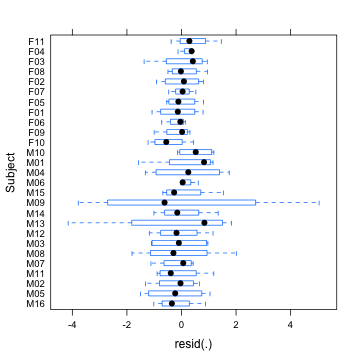
\includegraphics[width=\textwidth]{lectures/day_7_diagnostics_of_mems/figures/unnamed-chunk-36-1.png}
        \end{column}
        \begin{column}{0.5\textwidth}
        \normalsize
            Both M09 and M13 (two boys) have much larger variances than any of the other children, which is in line with the finding that boys have a larger residual variance than girls in their growth.
        \end{column}
    \end{columns}
\end{frame}

\begin{frame}[fragile]
    \frametitle{Observed versus fitted values by Subject}
    \scriptsize\begin{Verbatim}[numbers=left,numbersep=6pt,frame=single]
plot(fm1, distance ~ fitted(.) | Subject, abline = c(0,1))
    \end{Verbatim}
    \begin{columns}
        \begin{column}{0.6\textwidth}
            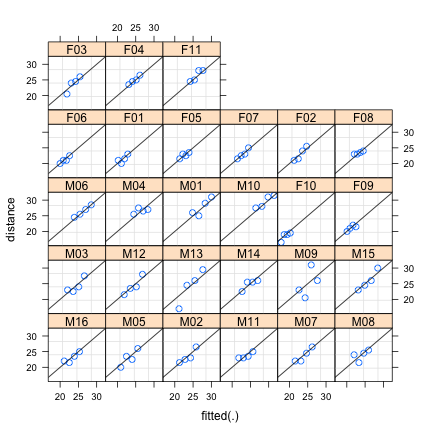
\includegraphics[width=\textwidth]{lectures/day_7_diagnostics_of_mems/figures/unnamed-chunk-37-1.png}
        \end{column}
        \begin{column}{0.4\textwidth}
        \normalsize
            Again we see that M09 and M13 have much larger variances than any of the other children.
        \end{column}
    \end{columns}
\end{frame}

\begin{frame}[fragile]
    \frametitle{Standardized residuals along age, separated by Subject}
    \scriptsize\begin{Verbatim}[numbers=left,numbersep=6pt,frame=single]
plot(fm1, resid(.) ~ age | Subject, abline = 0)
    \end{Verbatim}
    \begin{columns}
        \begin{column}{0.6\textwidth}
            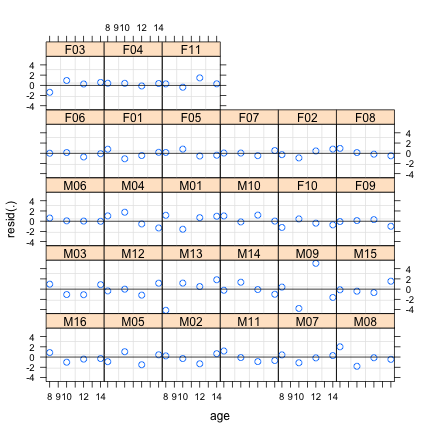
\includegraphics[width=\textwidth]{lectures/day_7_diagnostics_of_mems/figures/unnamed-chunk-38-1.png}
        \end{column}
        \begin{column}{0.4\textwidth}
        \normalsize
            Again observe the spread in M09 and M13 (in the latter, it is one data point)
        \end{column}
    \end{columns}
\end{frame}

\begin{frame}
    \frametitle{Modeling Within-Group Variance}
    \large
    We could now model the within-group/residual variance better by allowing each child its own variance (in contrast to the standard in LMEMs to assume the same variance within each level of a grouping variable)
    \vspace{0.5cm}
    
    \textit{More on Heterogeneuos Variance models using nlme():} \color{blue}\href{https://quantdev.ssri.psu.edu/sites/qdev/files/ILD_Ch06_2017_MLMwithHeterogeneousVariance.html}{here}
\end{frame}

\begin{frame}[fragile]
    \huge\color{purple}\textbf{Convergence issue checks with lme4}
\end{frame}

\begin{frame}[fragile]
    \frametitle{1. Check for Singularity: True}
    \scriptsize
    \begin{Verbatim}[numbers=left,numbersep=6pt,frame=single]
VarCorr(m.f)
    \end{Verbatim}[numbers=left,numbersep=6pt,frame=single]
    \scalebox{1}{
        \lstinputlisting[frame=single]{lectures/day_7_diagnostics_of_mems/outputs/output_13_1.txt}
    }
    \begin{Verbatim}[numbers=left,numbersep=6pt,frame=single]
isSingular(m.f)
---
[1] TRUE
    \end{Verbatim}

    \begin{Verbatim}[numbers=left,numbersep=6pt,frame=single]
VarCorr(m.f.2)
    \end{Verbatim}
    \scalebox{1}{
        \lstinputlisting[frame=single]{lectures/day_7_diagnostics_of_mems/outputs/output_13_2.txt}
    }
    \begin{Verbatim}[numbers=left,numbersep=6pt,frame=single]
isSingular(m.f.2)
---
[1] FALSE
    \end{Verbatim}
\end{frame}

\begin{frame}[fragile]
    \frametitle{2. Action: Scale Predictors}
    \begin{equation*}
        scale(\mathbf{x}) = \frac{\mathbf{x} - mean(\mathbf{x})}{sd(\mathbf{x})}
    \end{equation*}
    \vspace{0.3cm}
    
    \scriptsize
    \begin{Verbatim}[numbers=left,numbersep=6pt,frame=single]
m.f.scaled <- 
lmer(root ~ scale(week) * fertilizer + (scale(week)|plant), fertilizer)
VarCorr(m.f.scaled) 
    \end{Verbatim}
    \begin{Verbatim}[numbers=left,numbersep=6pt,frame=single]
 Groups   Name        Std.Dev. Corr 
 plant    (Intercept) 0.335781      
          scale(week) 0.076364 1.000
 Residual             0.466013
    \end{Verbatim}

    \begin{Verbatim}[numbers=left,numbersep=6pt,frame=single]
isSingular(m.f.scaled)
---
[1] TRUE
    \end{Verbatim}
    \normalsize That did not help...
\end{frame}

\begin{frame}[fragile]
    \frametitle{3. Specify Starting Values for Parameters}
    \scriptsize
    \begin{Verbatim}[numbers=left,numbersep=6pt,frame=single]
a <- getME(m.f,c("theta")) # re-param estimates
b <- getME(m.f,c("beta")) # fixed param estimates

m.check <- lmer(root ~ week * fertilizer + (week|plant), 
            data = fertilizer,
            start=list(theta=a,fixef=b))

isSingular(m.check)
    \end{Verbatim}
    \begin{Verbatim}[numbers=left,numbersep=6pt,frame=single]
[1] TRUE
    \end{Verbatim}
     \normalsize That did not help either...
    
\end{frame}

\begin{frame}[fragile]
    \frametitle{4. Compare Potential Optimizers}
    \scriptsize
    \begin{Verbatim}[numbers=left,numbersep=6pt,frame=single]
modelfit.all <- lme4::allFit(m.f)    
    \end{Verbatim}
    \begin{Verbatim}[numbers=left,numbersep=6pt,frame=single]
bobyqa : [OK]
Nelder_Mead : [OK]
nlminbwrap : [OK]
nmkbw : [OK]
optimx.L-BFGS-B : [OK]
nloptwrap.NLOPT_LN_NELDERMEAD : [OK]
nloptwrap.NLOPT_LN_BOBYQA : [OK]        
    \end{Verbatim}
\end{frame}

\begin{frame}
    \frametitle{Residual Simulations}
    - Simulate responses under the postulated model.
    - Repeat the process many times.
    - Create a distribution of simulated residuals and compare to observed residuals.
\end{frame}

\begin{frame}[fragile]
    \frametitle{Residual Simulations with DHARMa}
    \lstset{style=Rstyle}
    \begin{lstlisting}
    library(DHARMa)
    \end{lstlisting}
    \begin{itemize}
        \item DHARMa package documentation: \href{https://cran.r-project.org/web/packages/DHARMa/vignettes/DHARMa.html}{here}.
    \end{itemize}
\end{frame}

\begin{frame}
    \frametitle{Recap of Day 8}
    \begin{itemize}
        \item Diagnose Linear Mixed Effects Models by checking variance components, random effects, and residuals.
        \item Plot residuals for unique random effects levels and consider complex R-side and G-side matrices.
    \end{itemize}
\end{frame}

\end{document}